\subsubsection{Aggressive Optimizations (\texttt{-O3})}\label{subsec:seq_3}

The adoption of the \texttt{-O3} optimization level produces a dramatic shift in the performance profile of the kernel. At this stage, the compiler goes beyond conservative instruction scheduling and actively restructures the execution pattern to overcome the severe bandwidth bottlenecks caused by poor cache utilization.

\begin{figure}[H]
\centering
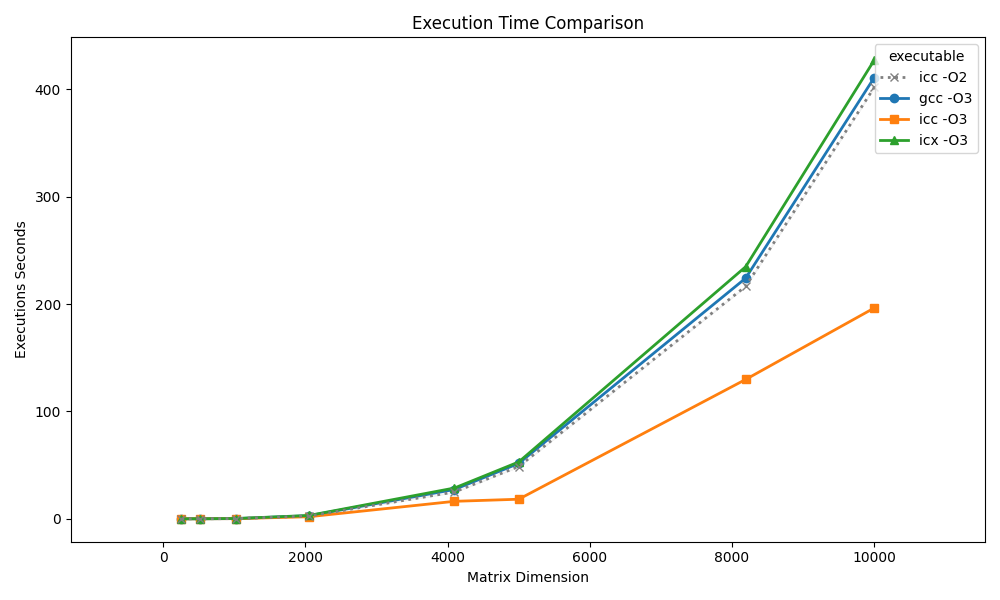
\includegraphics[width=0.8\textwidth]{Images/all_o3.png}
\caption{All compilers -O3 performances compared to ICC -O2}
\label{fig:all_o3}
\end{figure}


\paragraph{Compiler Optimization Report}
The ICC optimization report reveals that the compiler has fundamentally refactored the triple-nested loop into a complex, multi-level structure\footnote{See Appendix~\ref{subsec:tiling} for an in-depth explanation of how the \emph{Tiling Algorithm} works.}.

\begin{lstlisting}[style=CStyle, caption={Refactored ICC Optimization Report for \texttt{-O3}.}]
LOOP BEGIN (i-tile)
    LOOP BEGIN (k-tile)
        LOOP BEGIN (j-tile)
            LOOP BEGIN (i-inner) blocked by 128
                LOOP BEGIN (k-inner) blocked by 128
                    1. LOOP BEGIN (j-peeled)
                    2. LOOP BEGIN (j-vectorized)
                         remark #15388: aligned access
                         remark #15305: vector length 2, unroll factor 4
                         remark #15300: LOOP WAS VECTORIZED
                    3. LOOP BEGIN (j-alternate-alignment)
                    4. LOOP BEGIN (j-remainder)
                         remark #15335: loop not vectorize
                LOOP END
            LOOP END
        LOOP END
    LOOP END
LOOP END
\end{lstlisting}


\paragraph{Intel Advisor Roofline Analysis}
The structural changes translate directly into a massive throughput increase, as shown in the Roofline model (Figure~\ref{fig:icc_O3_roofline}).

\begin{figure}[H]
\centering
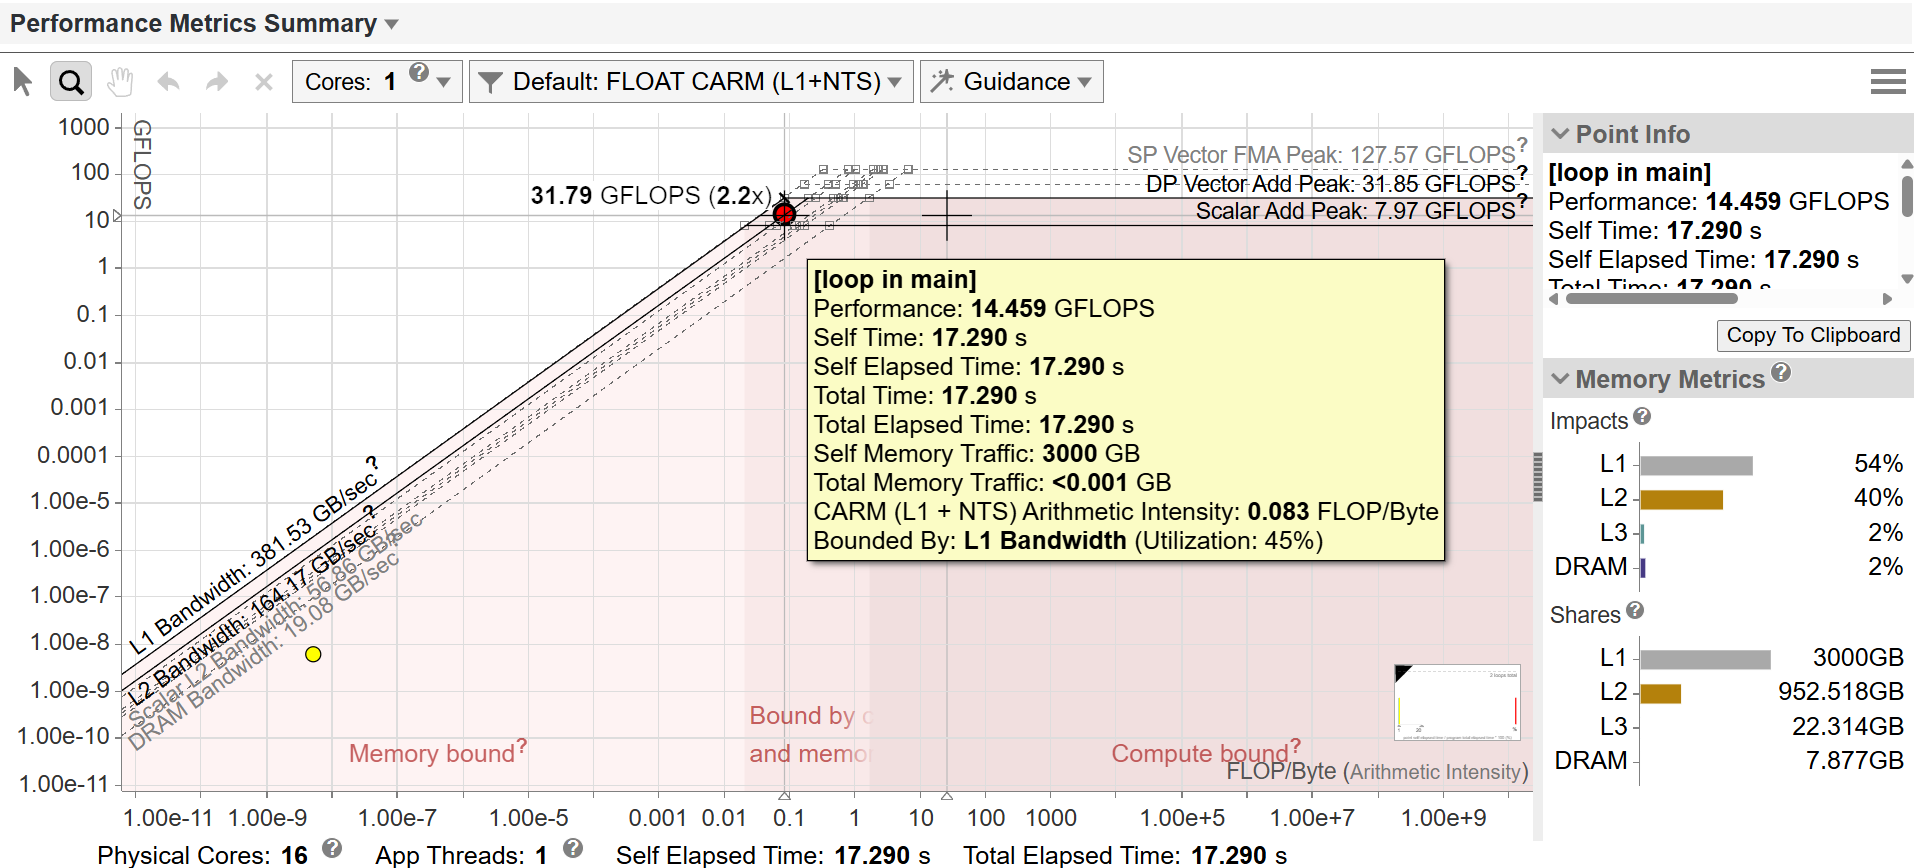
\includegraphics[width=\textwidth]{Images/ICC_O3_Roofline.png}
\caption{Roofline analysis for ICC \texttt{-O3}.}
\label{fig:icc_O3_roofline}
\end{figure}

The kernel achieves a computational throughput of \textbf{14.459 GFLOPS}, a significant uplift from \texttt{-O2} (that performed 6.062 GFLOPS). 

Observe how the \textbf{Arithmetic Intensity (AI)} keep the same value as the previous optimization at $0.083$ FLOP/Byte: this confirms that the performance gain is not due to doing "less memory work" per operation, but rather doing that work much faster by shifting the bottleneck.

The kernel's operational point has exceeded the scalar add peak, moving toward the vector add peak; the bottleneck is now  \textbf{L1 Bandwidth Bound} (saturating 45\% of maximum capacity). 

The decomposition of execution time shows that the L1 cache (54\%) and L2 cache (40\%) are the primary bottlenecks, while DRAM impact is negligible. 

This proves the tiling was successful: the data is now almost entirely encapsulated within the smaller (and faster) caches.

\paragraph{Valgrind Cachegrind Analysis}

The efficacy of the tiling is quantitatively confirmed by the memory profiling in Table~\ref{tab:cachegrind_results_o3}.

\begin{table}[H]
\centering
\caption{Key Valgrind Cachegrind metrics for ICC \texttt{-O3}.}
\label{tab:cachegrind_results_o3}
\begin{tabular}{lr}
\toprule
\textbf{Metric} & \textbf{Total Count / Rate} \\
\midrule
Instruction References (I) & 297,143,584,210 \\
Data References (D)        & 187,582,341,902 \\
\midrule
L1 Data Miss Rate          & \textbf{8.9\%} \\
Last-Level (LL) Miss Rate  & \textbf{0.1\%} \\
\bottomrule
\end{tabular}
\end{table}

The L1D miss rate has dropped significantly to 8.9\%, indicating much better temporal locality. Most importantly, the L3 miss rate is near-zero (0.1\%). This demonstrates that despite the large matrix size, the optimized access pattern ensures that almost no data requests need to traverse the hierarchy to the DRAM. The high degree of data reuse within the primary and secondary caches allows the CPU to sustain much higher GFLOPS by avoiding the high-latency penalty of main memory.